\documentclass[border=10pt]{standalone}

\usepackage{tikz}
\usepackage{tikzsymbols}
\usetikzlibrary{calc,patterns,shapes.geometric}

\def\centerarc[#1](#2)(#3:#4:#5){\draw[#1] ($(#2)+({#5*cos(#3)},{#5*sin(#3)})$) arc (#3:#4:#5);}

\begin{document}
	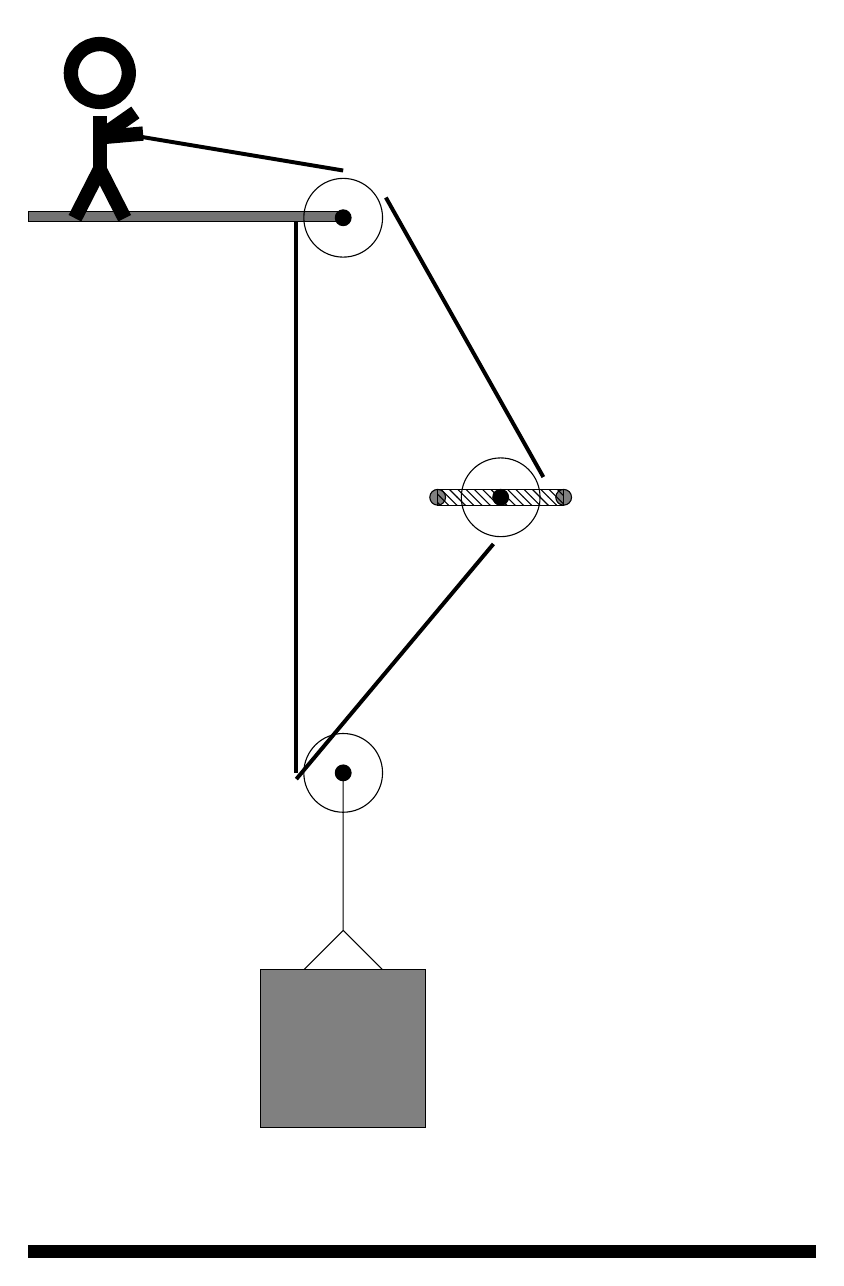
\begin{tikzpicture}
		%%%%% START %%%%%
		\draw[fill=black!55] (-2, 10) rectangle (2, 10.125);
		
		\draw (2, 3.0) circle (0.5);
		\draw[fill=black] (2, 3.0) circle (0.1);
		
		\draw (2, 10.05) circle (0.5);
		\draw[fill=black] (2, 10.05) circle (0.1);
		
		\draw[fill=white](4, 6.5) circle (0.5);
		\draw[fill=black] (4, 6.5) circle (0.1);
		\draw[fill=black!50] (3.2, 6.5) circle (0.1);
		\draw[fill=black!50] (4.8, 6.5) circle (0.1);
		\draw[pattern=north west lines, pattern color=black] (3.2, 6.6) rectangle (4.8, 6.4);
		
		\draw (2, 3.0) -- (2, 1.0) -- (1.5, 0.5) -- (2.5, 0.5) -- (2, 1.0);
		\draw[fill=black!50] (0.95, 0.5) rectangle (3.05, -1.5);
		
		\draw[line width=0.5mm] (1.4, 10) -- (1.4, 3.0);
		\centerarc[line width=0.5mm](2, 3.0)(180:330:0.6);
		\draw[line width=0.5mm](1.405, 2.921) -- (3.908, 5.907);
		\centerarc[line width=0.5mm](4, 6.5)(390:325:0.6);
		\draw[line width=0.5mm](4.542, 6.757) -- (2.542, 10.307);
		\centerarc[line width=0.5mm](2, 10.05)(30:90:0.6);
		\draw[line width=0.5mm](2, 10.65) -- (-1, 11.15);
		
		\node at (-1, 11.15) {\Strichmaxerl[10][-175][35]};
		
		\draw[fill=black] (-2, -3) rectangle (8, -3.15);
		%%%%% END %%%%%
	\end{tikzpicture}
\end{document}